\newpage
\subsection{GLINT driver}
\subsubsection{Overview}
%
GLINT is the most complex of the drivers supplied as part of GLIMMER. It was
originally developed as an interface between GLIDE and the GENIE Earth-system
model, but is designed to be flexible enough to be used with a wide range of
global climate models. Perhaps the most distinctive feature of GLINT is the
way it uses the object-oriented GLIDE architecture to enable multiple ice
models to be coupled to the same climate model. This means that regional ice
models can be run at high resolution over several parts of the globe, but
without the expense of running a global ice model.

GLINT automates the processes required in coupling regional models to a global
model, particularly the down- and up-scaling of the fields that form the
interface between the two models. The user may specify map projection
parameters for each of the ice models (known as \emph{instances}), and choose
one of several alternative mass-balance schemes to use in the coupling. The
differing time-steps of global model, mass-balance scheme, and ice model are
handled automatically by temporal averaging or accumulation of quantities (as
appropriate). This is illustrated schematically in figure~\ref{ug.fig.glint_timesteps}.  
%
\begin{figure}[htbp]
  \centering
  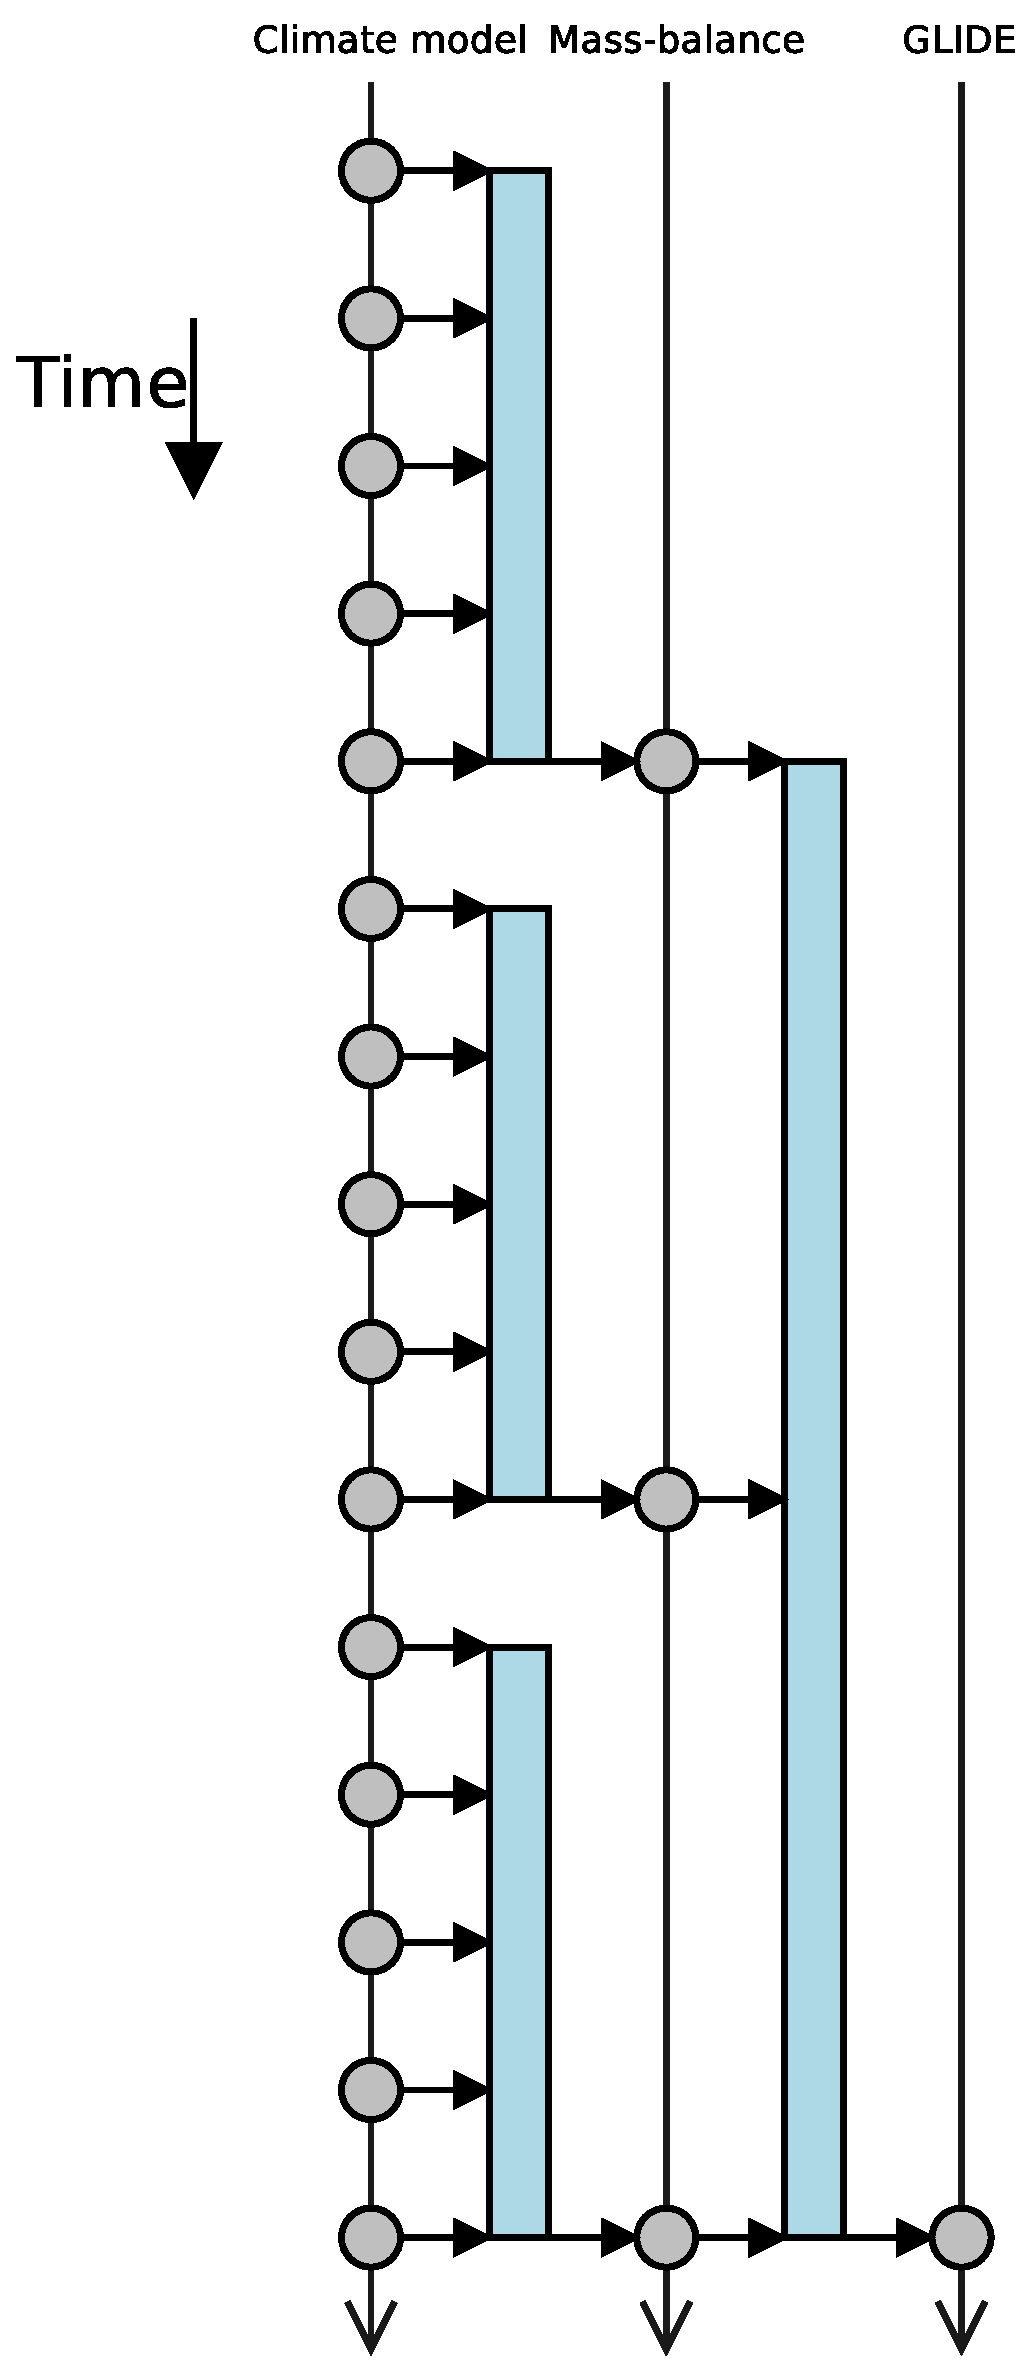
\includegraphics[width=0.6\textwidth]{\dir/figs/glint_timesteps.eps}
  \caption{Relationship between the timesteps in GLINT. The filled circles
  represent timesteps, the rectangles represent averaging/accumulation, and the arrows,
  flow of coupling fields.}
  \label{ug.fig.glint_timesteps}
\end{figure}
%
\subsubsection{Prerequisites}
%
If you plan to use GLINT, the following should be borne in mind:
%
\begin{itemize}
\item Global input fields must be supplied on a latitude-longitude
  grid. The grid does not have to be uniform in latitude, meaning that
  Gaussian grids may be used. Irregular grids (e.g. icosahedral grids) are not
  supported currently. The boundaries of the grid boxes may be specified; if
  not, they are assumed to lie half-way between the grid-points in lat-lon space.
\item In the global field arrays, latitude must be indexed from north to south
  -- i.e. the first row of the array is the northern-most one. Again, some
  flexibility might be introduced into this in the future.
\item The global grid must not have grid points at either of the
  poles. This restriction is not expected to be permanent, but in the meantime
  can probably be overcome by moving the location of the polar points to be
  fractionally short of the pole (e.g. at 89.9$^{\circ}$ and -89.9$^{\circ}$).
\end{itemize}
%
\subsubsection{Initialising and calling}

The easiest way to learn how GLINT is used is by way of an
example. GLINT should be built automatically as part of GLIMMER, and we assume
here that this has been achieved successfully.

Typically, GLINT will be called from the main program body of a
climate model. To make this possible, the compiler needs to be told to use the
GLINT code. Use statements appear at the very beginning of f90 program
units, before even \texttt{implicit none}:
%
\begin{verbatim}
  use glint_main
\end{verbatim}
%
The next task is to declare a variable of type \texttt{glint\_params}, which
holds everything relating to the model, including any number of ice-sheet
instances:
%
\begin{verbatim}
  type(glint_params) :: ice_sheet
\end{verbatim}
%
Before the ice-sheet model may be called from the climate model, it must be
initialised. This is done with the following subroutine call:
%
\begin{verbatim}
  call initialise_glint(ice_sheet,lats,lons,time_step,paramfile)
\end{verbatim}
%
In this call, the arguments are as follows:
%
\begin{itemize}
\item \texttt{ice\_sheet} is the variable of type \texttt{glint\_params}
 defined above;
\item \texttt{lats} and \texttt{lons} are one-dimensional arrays giving the
  locations of the global grid-points in latitude and longitude, respectively;
\item \texttt{time\_step} is the intended interval between calls to GLINT, in
hours. This is known as the \emph{forcing timestep}. 
\item \texttt{paramfile} is the name of the GLINT configuration file.
\end{itemize}
%
The contents of the configuration file will be dealt with later. Having
initialised the model, it may now be called as part of the main climate
model time-step loop:
%
\begin{verbatim}
    call glint(ice_sheet,time,temp,precip,orog)
\end{verbatim} 
%
The arguments given in this example are the compulsory ones only; a large number of
optional arguments may be specified -- these are detailed in the reference
section below. The compulsory arguments are:
%
\begin{itemize}
\item \texttt{ice\_sheet} is the variable of type \texttt{glint\_params}
 defined above;
\item \texttt{time} is the current model time, in hours;
\item \texttt{temp} is the daily mean $2\,\mathrm{m}$ global air temperature field, in
  $^{\circ}\mathrm{C}$;
\item \texttt{precip} is the global daily accumulated precipitation field,
  in $\mathrm{mm}$ (water equivalent, making no distinction
  between rain, snow, etc.);
\item \texttt{orog} is the global orography field, in $\mathrm{m}$.
\end{itemize}
%
Two mass-balance schemes, both based on the positive degree day (PDD) method,
are supplied with GLIMMER, and are available through GLINT. One of these calculates the mass-balance for the
whole year (the \emph{Annual PDD scheme}), while the other calculates on a
daily basis (the \emph{Daily PDD scheme}). The annual scheme incorporates a
stochastic temperature variation to account for diurnal and other variations,
which means that if this scheme is to be used, GLINT should be called such
that it sees a seasonal temperature variation which has had those variations
removed. In practice, this means calling GLINT on a monthly basis, with
monthly mean temperatures. For the daily scheme, no such restriction exists,
and the scheme should be called at least every 6 hours.
%
\subsubsection{Finishing off}
%
After the desired number of time-steps have been run, GLINT may have some
tidying up to do. To accomplish this, the subroutine \texttt{end\_glint}
must be called:
%
\begin{verbatim}
  call end_glint(ice_sheet)
\end{verbatim}
%
\subsubsection{API}
%
A detailed description of the GLINT API may be found in the appendices.
%
\subsubsection{Configuration}
%
GLINT uses the same configuration file format as the rest of GLIMMER. In the
case where only one GLIDE instance is used, all the configuration data for
GLINT and GLIDE can reside in the same file. Where two or more instances are
used, a top-level file specifies the number of model instances and the name of
a configuration file for each one. Possible configuration sections specific to
GLINT are as follows:
\begin{center}
  \tablefirsthead{%
    \hline
  }
  \tablehead{%
    \hline
    \multicolumn{2}{|p{0.98\textwidth}|}{\emph{\small continued from previous page}}\\
    \hline
  }
  \tabletail{%
    \hline
    \multicolumn{2}{|r|}{\emph{\small continued on next page}}\\
    \hline}
  \tablelasttail{\hline}
  \begin{supertabular}{|l|p{11cm}|}
%%%% 
    \hline
    \multicolumn{2}{|l|}{\texttt{[GLINT]}}\\
    \hline
    \multicolumn{2}{|p{0.98\textwidth}|}{Section specifying number of instances.}\\
    \hline
    \texttt{n\_instance} & (integer) Number of instances (default=1)\\
    \hline
%%%% 
    \hline
    \multicolumn{2}{|l|}{\texttt{[GLINT instance]}}\\
    \hline
    \multicolumn{2}{|p{0.98\textwidth}|}{Specifies the name of an
    instance-specific configuration file. Unnecessary if we only have one
    instance whose configuration data is in the main config file.}\\
    \hline
    \texttt{name} & Name of instance-sepcific config file (required).\\
    \hline
%%%% 
    \hline
    \multicolumn{2}{|l|}{\texttt{[GLINT climate]}}\\
    \hline
    \multicolumn{2}{|p{0.98\textwidth}|}{GLINT climate configuration}\\
    \hline
    \texttt{evolve\_ice} & {\raggedright
      specify whether or not the ice sheet evolves in time: \\
      \begin{tabular}{lp{10cm}}
        0 &  Do not evolve ice sheet (hold fixed in time)\\
        {\bf 1} & Allow the ice sheet to evolve \\
      \end{tabular}}\\
    \texttt{precip\_mode} & {\raggedright
      Method of precipitation downscaling: \\
      \begin{tabular}{lp{10cm}}
        {\bf 1} & Use large-scale precipitation rate\\
        2 & Use parameterization of \emph{Roe and Lindzen}\\
      \end{tabular}}\\
    \texttt{acab\_mode} & {\raggedright
      Mass-balance model to use:\\
      \begin{tabular}{lp{7cm}}
        {\bf 1} & Annual PDD mass-balance model (see section \ref{ug.mbal.pdd_scheme}) \\
        2 & Annual accumulation only\\
        3 & Hourly energy-balance model (RAPID - not yet available) \\
        4 & Daily PDD mass-balance model (no docs yet)\\
      \end{tabular}}\\
    \texttt{ice\_albedo} & Albedo of ice --- used for coupling to climate
    model (default=0.4) \\
    \texttt{lapse\_rate} & Atmospheric temperature lapse-rate, used to correct
    the atmospheric temperature onto the ice model orography. This should be
    \emph{positive} for temperature falling with height
    ($\mathrm{K}\,\mathrm{km}^{-1}$) (default=8.0) \\
    %%%%%%%%%%%%%%
    \texttt{data\_lapse\_rate} & Atmospheric temperature vertical lapse rate,
    to be used in the calculation of temperature at
    sea-level. The variable \texttt{lapse\_rate} is then used to adjust the
    temperature to the surface of the local ice sheet topography. If
    \texttt{data\_lapse\_rate} is not set, it is set to the value of
    \texttt{lapse\_rate} by default. \\
    %%%%%%%%%%%%%%
    \texttt{ice\_tstep\_multiply} & Ice time-step multiplier: allows
    asynchronous climate-ice coupling. See below for full explanation of GLINT
    time-stepping. (default = 1) \\
    %%%%%%%%%%%%%%
    \texttt{mbal\_accum\_time} & Mass-balance accumulation time (in years,
    default is equal to mass-balance timestep).  See below for full explanation of GLINT
    time-stepping. \\
    \hline
  \end{supertabular}
\end{center}

\subsubsection{GLINT timestepping --- an explanation}

By default, the model accepts input on each forcing timestep (as specified in 
the call to \texttt{initialise\_glint}, above). These are accumulated over the course 
of a mass-balance time-step, whereupon the mass-balance model is called. The 
output from the mass-balance model is accumulated over the course of an ice 
model time-step, and finally the ice model is called.

This default behaviour can be altered, in two ways:
\begin{enumerate}
\item The number of ice sheet time-steps executed for each accumulated 
mass-balance field may be increased - thus accelerating the icesheet relative 
to the forcing. To do this, set \texttt{ice\_tstep\_multiply} in the \texttt{[GLINT climate]} 
config section - must be an integer. This is only possible if the 
mass-balance is accumulated over an integer number of years.
\item The mass-balance accumulation period can be altered by setting  
\texttt{mbal\_accum\_time} in the \texttt{[GLINT climate]} config section --- this is a 
floating-point value in years.
\end{enumerate}

The interaction of these two parameters is fairly complex, and permits a 
reasonably sophisticated control of how the ice sheet model is forced. 
Various checks are made at run-time to make sure sensible/possible values are selected. Most 
importantly, all relevant time-steps must divide into one another 
appropriately - the model will (should\ldots) stop if an un-sensible combination 
of values is detected.

\subsubsection{GLINT timestepping --- further examples}

To aid understanding of the time-stepping controls, here are some examples. First, suppose we have these time-step values:

\vspace{0.5cm}
\begin{tabular}{ll}
forcing time-step: & 6 hours \\
mass-balance time-step: & 1 day \\
ice time-step: & 0.5 year
\end{tabular}
\vspace{0.5cm}

By default, the model will accumulate 6 months' worth of mass-balance 
calculations, and force the ice sheet model based on that. This might not be 
desirable, so you could set:

\begin{verbatim}
    mbal_accum_time = 1.0
\end{verbatim}

This would make GLINT accumulate 1 year's worth of mass-balance output before 
forcing the ice sheet (at which point it would execute \emph{two} ice sheet 
time-steps of 0.5 years each).

Having done that, you could accelerate the ice model by a factor of ten, by 
setting:

\begin{verbatim}
    ice_tstep_multiply = 10
\end{verbatim}

In this scenario, 20 ice sheet time-steps of 0.5 years each would be done 
after each 12-month accumulation of mass-balance data.

For the second example, we consider the contrasting situation where we don't want to calculate a 
mass-balance on all the available data (perhaps to save time). Consider 
these time-step values:

\vspace{0.5cm}
\begin{tabular}{ll}
forcing time-step:   &   6 hours \\
mass-balance time-step: & 1 day \\
ice time-step:       &   10 years
\end{tabular}
\vspace{0.5cm}

(Clearly this a fairly numerically stable and/or low-resolution ice sheet).

To avoid running the daily PDD scheme c.3600 times (depending on the value of 
\texttt{days\_in\_year}), we can set to only use the first two years of data:

\begin{verbatim}
    mbal_accum_time = 2.0
\end{verbatim}

GLINT accumulates mass-balance for 2 years, then waits for 8 years (incoming 
data are ignored during this time), before calling the ice sheet. Ice sheet 
acceleration may be enabled with \texttt{ice\_tstep\_multiply} as before.
